% !TEX root = ../my-thesis.tex
%
\chapter{IMPLEMENTACIÓN DESARROLLADA}
\label{sec:implementación}

A lo largo de este capítulo, se desarrollará y explicará como se ha realizado la implementación de los diferentes algoritmos, que harán posible desarrollar posteriormente las pruebas y experimentos pertinentes para la verificación de la hipótesis y solución del problema que se desarrolla en este trabajo.

\section{Algoritmo Genético}

En primer lugar, se va a pasar a desarrollar como se ha realizado la elaboración del algoritmo genético, el cual tiene como fin optimizar la arquitectura de las redes de neuronales convolucionales.

Esto se realizará por medio de la librería elaborada en Python, \textbf{DEAP} (\textit{Distributed Evolutionary Algorithms in Python}) \footnote{\url{https://deap.readthedocs.io/en/master/}}. Esta es una librería ampliamente utilizada para el desarrollo de algoritmos evolutivos, como se puede ver en su página web. Esto es debido a su gran personalización y a la gran cantidad de representaciones aceptadas y algoritmos implementados dentro de la librería.

Se ha seleccionado esta librería mayoritariamente por su filosofía, ya que en vez de emplear inicializadores cerrados como en otras librerías disponibles, se nos solicita explícitamente cada uno de los parámetros del algoritmos, que son además, fácilmente modificables e integrables con el resto del software, adaptándose adecuadamente al problema que se trata de resolver. Además, el algoritmo esta totalmente disponible para su modificación, en caso de querer o requerir establecer una dinámica única del algoritmo evolutivo.

En este caso se va a partir de la implementación realizada en esta librería para un algoritmo genético de objetivo único, el cual, como se verá a lo largo de este capítulo, sufrirá de algunos cambios para realizar la ejecución de manera adecuada para resolver el problema dado.

Este va a seguir la estructura mostrada en la figura \ref{fig:esquema_funcional_GA}, y se desarrollarán cada uno de sus puntos a lo largo de este capítulo.\\

\begin{figure} [h]
    \centering
    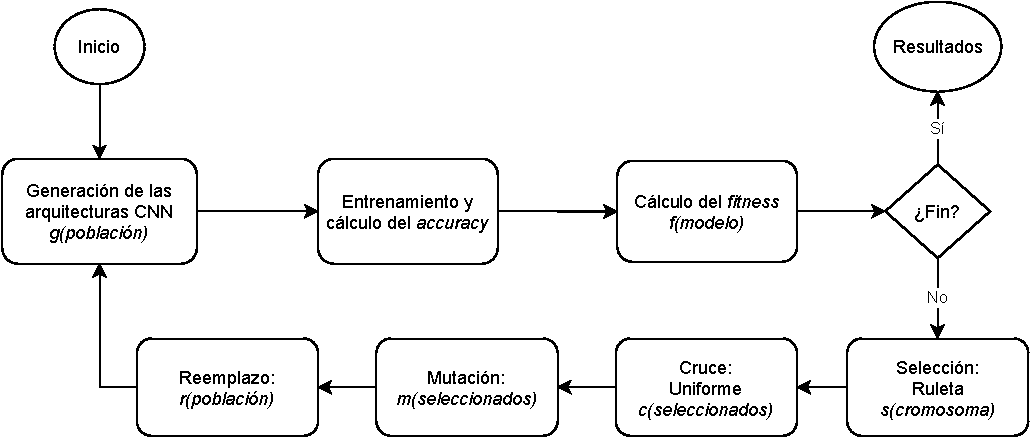
\includegraphics[width=\textwidth]{figuras/implementacion/esquema_funcionamiento.pdf}
    \caption{Esquema de funcionamiento de la implementación desarrollada del Algoritmo Genético}
    \label{fig:esquema_funcional_GA}
\end{figure}

\subsection{Codificación del problema}

La codificación del problema es uno de los puntos más delicados a la hora de desarrollar el algoritmo genético en cuestión como ya se ha visto en el desarrollo teórico.

En este caso, se ha planteado una codificación binaria basada en la selección de diferentes parámetros y configuraciones para cada una de las capas que conforman la arquitectura de la red neuronal convolucional.

Para ello, se ha seleccionado una codificación de \textbf{10 bits} para cada una de las capas de la red, donde se configurarán cada una de las propiedades que tiene esta. Posteriormente, cada una de estas capas de concatenarán formando finalmente la arquitectura de la red completa, donde como parámetro del algoritmo se deberá especificar el número de capas que formarán la arquitectura de la red definitiva.\\

\begin{table}[h]
\caption{Codificación de una capa de la CNN para el Algoritmo Genético}
\label{tab:codificacion}
\centering
\begin{tabular}{l|llllllllll}
\toprule
\textbf{Tipo}               & \multicolumn{10}{c}{\textbf{Posición de los genes}}                         \\
\textbf{de capa}            & \textbf{0} & \textbf{1} & \textbf{2}     & \textbf{3}     & \textbf{4}     & \textbf{5}     & \textbf{6}      & \textbf{7}      & \textbf{8}    & \textbf{9} \\ \hline
\textit{Vacía}              & 0 & 0 & x     & x     & x     & x     & x      & x      & x    & x \\
\textit{Pooling}            & 0 & 1 & $T$     & $K$     & x     & x     & x      & x      & x    & $S$ \\
\textit{Convolucional}        & 1 & 0 & $K_{x1}$ & $K_{x2}$ & $K_{y1}$ & $K_{y2}$ & $FMS_1$ & $FMS_2$ & $A_T$ & $S$ \\
\textit{Convolucional Residual} & 1 & 1 & $K_{x1}$ & $K_{x2}$ & $K_{y1}$ & $K_{y2}$ & $FMS_1$ & $FMS_2$ & $A_T$ & $S$ \\
\bottomrule
\end{tabular}
\end{table}

En la Tabla \ref{tab:codificacion}, se puede observar como es el esquema de codificación de cada una de las capas de la red neuronal. En ella se puede observar como se componen cada una de estas capas, donde se distinguen cuatro tipos de capas: \textit{Vacía}, \textit{Pooling}, \textit{Convolucional} y \textit{Convolucional Residual}. Estas vienen codificadas por dos genes que marcan el tipo de capa, que son las dos primeras que se encuentras en la codificación del problema.

Esta codificación además cuenta con numerosas ventajas, como el poder implementar redes anteriormente presentadas tales como VGG-16 y ResNet-50 como posibles individuos en la población, o de otra forma, de ser las mejores arquitecturas en el espacio de búsqueda, aparecer como solución.

A continuación, se va a pasar a desarrollar cuál es el significado de cada uno de los parámetros de cada tipo de capa que forman el genotipo del Algoritmo Genético propuesto.

\begin{itemize}
    \item \textbf{Capa vacía:} Esta tipo de capa es la más simple, y se implementa para poder codificar arquitecturas de diferente profundidad de capas. Es por ello que en la concatenación de capas puede aparecer una capa vacía la cuál no realizará ningún proceso, por lo que se podrán generar arquitecturas con menor número de capas que las seleccionadas.
    
    \item \textbf{\textit{Capa de Pooling}:} Esta se trata de una capa de tipo \textit{Pooling} como las que se presentaron en las bases teóricas del trabajo. Esta consta de tres parámetros principales para su configuración, que son: $T$, $K$ y $S$, que a continuación se pasará a su explicación.
    
    \begin{itemize}
        \item \textit{Tipo de Pooling} ($T$) :  Este parámetro hace referencia al tipo de operación de \textit{Pooling} que se va a realizar en esta capa. Se han seleccionado dos operaciones posibles para esta capa que son: \textbf{\textit{Average Pooling}} y \textbf{\textit{Max Pooling}}.
        
        \item \textit{Tamaño del filtro (kernel)} ($K$) : Este parámetro hace referencia al tamaño del filtro que se introducirá en esta operación. Este tendrá un tamaño cuadrado y un tamaño de \textbf{2 o 3 píxeles}.
        
        \item \textit{Stride} ($S$) : Este hace referencia al paso con el que se va recorriendo el filtro o \textit{kernel} a lo largo de la imagen de entrada. Se pueden dar dos casos, que se realice son \textit{stride} de \textbf{2 o de 3 píxeles}.
        
    \end{itemize}
    
    Como se puede observar, empleando este tipo de codificación, es posible que en algunos casos se de la problemática de situarse varias capas de \textit{Pooling} de forma consecutiva, cosa que no tiene sentido a la hora de generar la estructura de la red. Es por ello que, de producirse numerosas capas de este tipo de forma seguida, solo se tendrá en cuenta la primera, ignorándose las siguientes capas de \textit{Pooling} que vayan apareciendo posteriormente.
    
    \item \textbf{Capa Convolucional:} Esta se trata de una capa convolucional. Esta es algo más compleja que lo que se veía para las capas de tipo \textit{Pooling} ya que existen muchos más parámetros ajustables dentro de ellas, y muchas más combinaciones como se pueden ver por ejemplo en las redes VGG-16 o ResNet-50. 
    
    Otra puntualización, es que en este tipo de capas, el tamaño del filtro puede ser asimétrico como sucede por ejemplo en las redes con bloques de tipo Inception. Para dar mayores posibilidades a las arquitecturas que se pueden generar, se introducirá de la misma manera la posibilidad de codificar este tipo de filtros asimétricos.
    
    Esta capa convolucional se puede configurar por un mayor número de parámetros que otras redes y estas vienen codificadas por los parámetros: $K_{x}$, $K_{y}$, $FMS$, $A_T$ y $S$, que a continuación van a ser explicados.
    
    \begin{itemize}
        \item \textit{Tamaño del filtro en dirección horizontal} ($K_{x}$) : Hace referencia dentro de la capa convolucional seleccionada, al tamaño en dirección horizontal que puede tomar el filtro. Este consta de 2 bits para su codificación, por lo que se pueden generar hasta cuatro combinaciones de tamaños. El tamaño final, por tanto viene dado por la siguiente expresión:
        
        \begin{equation}
            \textit{Kernel Size} = \text{dec}(K_x) \cdot 2 + 1
        \end{equation}
        
        dando como resultado, la posibilidad codificar tamaños filtros de \textbf{1, 3, 5 y 7}.
        
        \item \textit{Tamaño del filtro en dirección vertical} ($K_{y}$) : Este funciona de manera análoga a como lo hace $K_x$ sin diferencia ninguna a la hora de codificar los tamaños de los filtros. La única diferencia radica a que se hace referencia al tamaño del filtro en dirección vertical, consiguiendo de esta manera poder codificar tamaños de filtros no cuadrados.
        
        \item \textit{Número de filtros (Feature Map Size)} ($FMS$) : Este parámetro hace referencia al número de filtros que existirán en cada una de las capas de convolución. Un mayor número de estos, obtendrán mayor cantidad de detalles de la imagen, a cambio de hacer mucho más lenta y pesada esta red, si esta es demasiado voluminosa en las capas iniciales de la red, donde el tamaño de entrada de la imagen aún es demasiado grande. Es por ello que se da la selección entre diferentes posibilidades de números de filtros en esta capa.
        
        Para determinar el número de filtros que tendrá una capa es necesario a partir de la codificación de 2 bits, aplicar las siguientes expresiones:
        
        \begin{equation}
            \textit{Feature Map Size} = 2^P
        \end{equation}
        
        \begin{equation}
            P = \text{dec}(FMS) + 6
        \end{equation}
        
        dando como resultado número de filtros posibles de \textbf{64, 128, 256 y 512}.
        
        \item \textit{Tipo de Función Activación} ($A_T$) : Este parámetro hace referencia al tipo de activación que usará posteriormente de haber realizado el proceso de convolución. Para ello existen dos opciones de función de activación: \textbf{\textit{ReLU}} y \textbf{\textit{tanh}}.
        
        \item \textit{Stride} ($S$) : Este es análogo al \textit{stride} que se encontraba en la capa de \textit{Pooling}. Aún así, para este caso cada uno de los bits hacen referencia a pasos diferentes, siendo en una capa de convolución de \textbf{1 o 2 píxeles}. Se ha seleccionado de esta manera para poder imitar el comportamiento de ResNet que huye del uso de capas de \textit{Pooling} y realiza la compresión de la imagen mediante capas de convolución con tamaños de \textit{stride} de 2.
        
    \end{itemize}
    
    Finalmente, tras la generación de cada capa de convolución, se añadirá una capa adicional de \textit{Batch Normalization} \cite{ioffe2015batch} que reduce de forma significativa el tiempo necesario de entrenamiento de la red. De igual manera, para mantener el tamaño de la imagen de entrada al realizar la convolución, es necesario introducir una capa de \textit{Padding} que seguirá la expresión:
    
    \begin{equation}
        P = \frac{K - 1}{2}
    \end{equation}
    
    \item \textbf{Capa Convolucional Residual:} Por último presentar las capas de tipo convolucional residual \cite{He2016}, que vienen introducidas para ayudar al aumento de la profundidad del modelo sin perder el contexto inicial de la imagen y por tanto, la facilidad de entrenamiento de la red.
    
    Los parámetros de configuración de este tipo de capas es exactamente igual especificado para capas convolucionales clásicas. Sin embargo, se deja un lazo abierto justo al crear esta capa que posteriormente será cerrada. Esto sucederá cuando se añada una capa que cumpla los siguientes casos: se añada una nueva capa de \textit{Pooling}, se añada otra capa convolucional residual o se haya llegado al final de codificación.\\
    
    \begin{figure}[h]
    \centering
    \begin{subfigure}{0.8\textwidth}
        \centering
        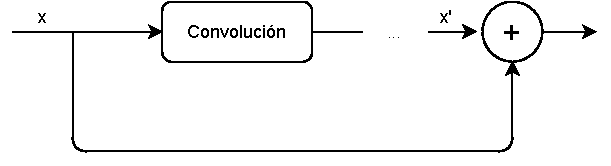
\includegraphics[width=\textwidth]{figuras/implementacion/Skip_convolucion_Implementacion_1.pdf}
        \caption{Capa Residual Identidad}
        \label{fig:residual_identidad}
    \end{subfigure}
    \hfill
    \begin{subfigure}{0.8\textwidth}
        \centering
        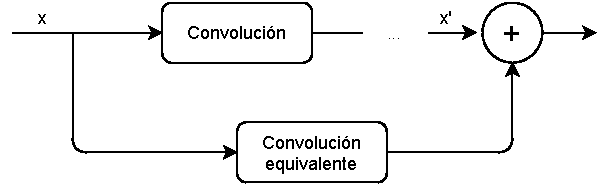
\includegraphics[width=\textwidth]{figuras/implementacion/Skip_convolucion_Implementacion_2.pdf}
        \caption{Capa Residual con capa extra de convolución para satisfacer tamaño de salida}
        \label{fig:residual_conv_eq}
    \end{subfigure}
    \caption{Representación de las posibles configuraciones de capas residuales}
    \label{fig:residual}
    \end{figure}
    
    Debido a la aleatoriedad de generación de este tipo de capas y sobretodo, cuando van a ser cerradas, es posible que se generen tamaños a la hora de realizar la operación de suma o \textit{addition}, que no pueden ser realizados. Para ello se propone la solución que se muestra en la Figura \ref{fig:residual}, donde como se puede observar, en caso de que el tamaño de la imagen \textit{x} sea diferente al tamaño de la imagen \textit{x'}, se genera una convolución equivalente para adaptar este tamaño en la rama residual.
    

\end{itemize}

\subsection{Función \textit{Fitness}}

Tras la generación de la arquitectura de la Red Neuronal Convolucional completa, es necesario realizar una evaluación del desempeño de esta con respecto a los otros individuos de la población, de tal manera que sea posible comparar que tan buena capacidad de clasificación tiene esta. A este valor o número se le denomina \textit{fitness}, como ya se veía en el apartado de las bases teóricas.

Existen diferentes parámetros que consiguen evaluar que tal es rendimiento de la red para la tarea de clasificación de cierto conjunto de datos de prueba etiquetados tras su entrenamiento. Entre ellos, se ha de seleccionar uno o la combinación entre varios, a través de la definición de una expresión entre ellos, que generarán el valor final de \textit{fitness}.

Se ha optado por seleccionar el parámetro \textit{accuracy} del \textit{top 1} como valor de \textit{fitness}, ya que es de los parámetros más extendidos para la comparación y evaluación del desempeño de la redes. Este también es denominado \textit{categorical accuracy} y es el empleado para problemas de clasificación de tipo multi-clase, como el problema que se está resolviendo. Esta se define como:

\begin{equation}
    \text{Accuracy} = \frac{\text{Número de predicciones correctas}}{\text{Número total de predicciones}}
\end{equation}

Además, durante el entrenamiento de las redes, se persigue en obtener el mayor valor de \textit{accuracy} posible, por lo que es adecuado clasificar nuestras redes por este indicador y no por otros como pudieran ser \textit{Precision}, \textit{F1-score} o \textit{Recall}.

\subsection{Selección}

Una vez establecidas las bases del problema en el Algoritmo Genético, se establecerán los diferentes operadores que modificarán a la población a lo largo de numerosas generaciones para conseguir a los mejores individuos.

En primer lugar se va a establecer la operación de selección de los padres que generará a la nueva población. Para ello se ha implementado una operación que se basa en el valor de \textit{fitness} obtenido durante su entrenamiento, dando mayor prioridad a reproducirse a los mejores individuos de la población, pero siempre tratando de conservar a los que podrían llevar algo de carga genética valiosa a pesar de obtener valores de \textit{fitness} menores. Esto asegura que se puedan obtener individuos mejores y además siempre haya oportunidad de explorar de forma uniforme el espacio de búsqueda de las soluciones.

La operación que se ha introducido en particular para esta implementación y que tiene el funcionamiento buscado, es el ya explicado \textbf{Selección por Ruleta} (\textit{Roulette Selection}). Por otro lado, se ha seleccionado una probabilidad de cruce del 90\% tratando de que exista gran cantidad de transpaso de información genética a lo largo de las diferentes generaciones.

\subsection{Cruce}

Una vez seleccionado los pares de individuos, se debe buscar realizar una combinación entre estos que transfiera información valiosa generando nuevos individuos con las propiedades de sus antecesores. Esto se hace mediante la aplicación del cruce como ya se explicó.

En este punto, es necesario ir con cautela a la hora de seleccionar el operador de cruce adecuado, ya que la selección de un mal operador, podría llevar a no generar una alta diversidad de población o que su evolución sea demasiado lenta. Es por ello que se descarta el uso de operadores de cruce tales como el \textit{Single-Point Crossover} o el \textit{Double-Point Crossover}, debido a que no generan gran diversidad en la población resultante.

Por tanto, para el operador cruce se propone el uso del operador de cruce, \textbf{\textit{Uniform Crossover}} que ya se explicó en anteriores capítulos. Este va a transferir información valiosa entre los individuos de forma uniforme a lo largo del genotipo, lo cual lo hace ideal. Se ha seleccionado a su vez una probabilidad de intercambio genético del 20\%, debido a que se debe asegurar que se transfieren parámetros realmente importantes a lo largo de la codificación, y estos resultan ser los dos primeros que seleccionan el tipo de cada capa. Estas resultan ser el 20\% de la codificación total del genotipo.

\subsection{Mutación}

En la operación de mutación, como se ha visto en la teoría, trata de realizar búsquedas de forma aleatoria dentro del espacio de búsqueda, de manera se evite localizarse en óptimos locales a lo largo de esta. Para esta se ha de seleccionar una probabilidad de mutación para cada individuo en cada generación, que decidirá si se le aplica este operador o no. Este ha de ser lo suficientemente bajo para no convertir esta búsqueda, en una búsqueda meramente aleatoria. Es por ello que se ha seleccionado una probabilidad de mutación del 5\%.

Para la selección del operador, al igual que sucedía con la operación de cruce, la mutación se va a realizar de forma uniforme a lo largo de todo el genotipo con una probabilidad de mutación dada. Esta se ha seleccionado de un valor del 20\%, ya que de manera análoga a lo que sucedía en el cruce, este debe ser un valor que asegure que en las pocas veces que se va a producir una mutación, se haga de manera adecuada, y permita un búsqueda en nuevas zonas del espacio de búsqueda de soluciones.

\subsection{Reemplazo}

Finalmente, se da la operación de reemplazo, la cuál se ha implementado una solución bastante sencilla, de manera que se combinan el total de nuevos individuos generados en la nueva generación junto a los individuos de la anterior población ordenados por valor de su \textit{fitness}. De esta lista ordenada, se toman los N valores fijos de población establecidos, que pasarán a ser los nuevos individuos de la nueva población para la siguiente generación.

\subsection{Elitismo}

Debido a la naturaleza del problema y como se ve alterada el \textit{fitness} en función de su correcta evaluación, es necesario asegurar una estrategia de Algoritmo Genético con elitismo. Esto es debido a que el \textit{fitness} se evalúa mediante un proceso de optimización, es posible que no se vea el verdadero potencial de los genes que contiene la arquitectura generada, por lo que se deberá tratar de conservar en su gran medida para asegurar que una vez encontrados un buen genotipo, este no se pierda a lo largo de las generaciones.

Esto se realiza, como ya se explicaba en las bases teóricas, para asegurar que no se pierde al mejor individuo y a su material genético a lo largo de las diferentes poblaciones. Esto unido a los elevados tiempos de ejecución de este tipo de algoritmo, ayuda a una convergencia, aunque sea local, mucho más rápida que si no se tuviera implementado este.

Debido a que la librería DEAP que ha sido la seleccionada para el desarrollo de los Algoritmos Genéticos, no implementa el mecanismo de elitismo de forma nativa, por lo que se ha realizado una modificación en la implementación para añadir este. Para ello, en el proceso de selección, se genera un individuo menos de los que se deberían seleccionar, y finalmente en el proceso de reemplazo, se añade a este individuo dentro de la población nuevamente de forma inalterada.


\section{Redes Neuronales Convolucionales}

Puesto que para analizar la capacidad de clasificación que tiene cada uno de las Redes Neuronales Convolucionales como individuo de la población es necesario realizar un proceso de entrenamiento y de prueba, en esta sección, se desarrollarán las configuraciones que se han realizado para el desempeño de estas redes.

Para realizar la implementación de esta parte, se ha hecho uso de las famosas librerías \textbf{Tensorflow} \cite{tensorflow} y \textbf{Keras} \cite{keras}, desarrolladas por Google Brain y liberadas en 2015. Estas son de código abierto y de alto nivel, permitiendo crear y entrenar redes neuronales profundas. Las principales ventajas de usar estas es su sencillo uso en comparación con otras librerías menos extendidas, su gran modularidad y capacidad de configuración, debido a que se basa en sistema de creación por bloques, y por último, la facilidad de extensión para desarrollar nuevas arquitecturas y metodologías. Otro punto a favor de emplear estas librerías es su gran desarrollo y su amplia comunidad, la cuál solucionan errores y aportan nuevas características de formas bastante continua, junto a enorme cantidad de material didáctico con el que aprender a usarlo de manera adecuada.

\subsection{Conjunto de Datos (\textit{Dataset})}

Para realizar el entrenamiento y validación de las redes, se ha tomar un \textit{dataset} adecuado que permita comparar el desempeño de las arquitecturas generadas. Este ya fue presentado con anterioridad en el Capítulo \ref{sec:problema}, pero debido a las limitaciones computacionales existentes, no van a ser empleadas todos los datos de este.

Por simplificación del problema, se han tomado en total un subconjunto de datos formado por dos especies de plantas más el conjunto de negativos. Estas dos especies seleccionadas son: ``Chinee apple'' y ``Snake Weed''.


Estos conjuntos de datos, han sido equilibrados de tal manera que exista un balance proporcional entre conjunto de datos de malas hierbas y negativos, y que entre las malas hierbas, exista un número similar entre las distintas especies. Esto se hace de esta manera para evitar posibles sesgos asociados a una mala elección de la cantidad de cada tipo con la que se va a entrenar.

Además, para evitar problemas de \textit{overfitting}, el conjunto de imágenes de entrada, se les aplicará la técnica del \textit{Data Augmentation} \cite{perez2017effectiveness}, por la cuál se producirán imágenes con pequeñas distorsiones a las originales, para generar conjuntos de datos más grandes y diferentes a lo largo del entrenamiento. 

Esta imagen de entrada sufrirá modificaciones de re-escalado, adición de \textit{zoom}, realización de giros horizontales y de rotación, cambios en el brillo y modificación de los canales de color. En la Figura \ref{fig:datagen}, se pueden ver algunos ejemplos del resultado de la aplicación de esta técnica.\\

\begin{figure}[h]
\centering
    \begin{subfigure}{0.3\textwidth}
        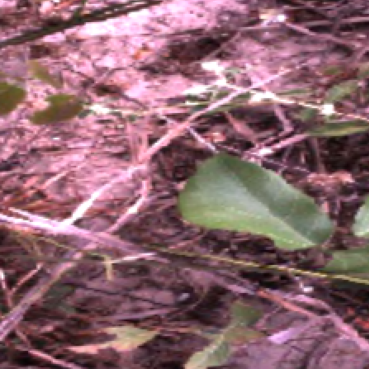
\includegraphics[width=\textwidth]{figuras/implementacion/dataset/imagenes_datagen_1.png}
        \caption{}
    \end{subfigure}
    \hfill
    \begin{subfigure}{0.3\textwidth}
        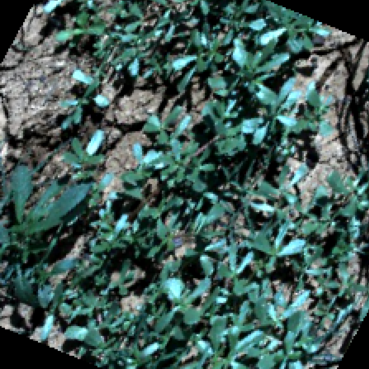
\includegraphics[width=\textwidth]{figuras/implementacion/dataset/imagenes_datagen_2.png}
        \caption{}
    \end{subfigure}
    \hfill
    \begin{subfigure}{0.3\textwidth}
        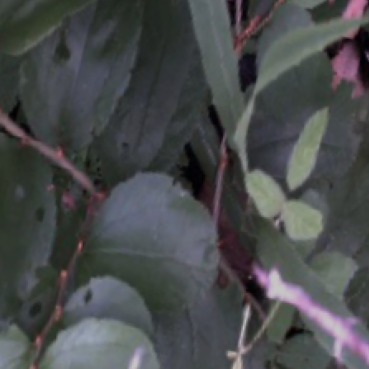
\includegraphics[width=\textwidth]{figuras/implementacion/dataset/imagenes_datagen_3.png}
        \caption{}
    \end{subfigure}
    \hfill
    \begin{subfigure}{0.3\textwidth}
        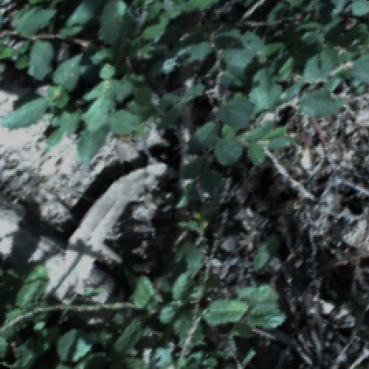
\includegraphics[width=\textwidth]{figuras/implementacion/dataset/imagenes_datagen_4.png}
        \caption{}
    \end{subfigure}
    \hfill
    \begin{subfigure}{0.3\textwidth}
        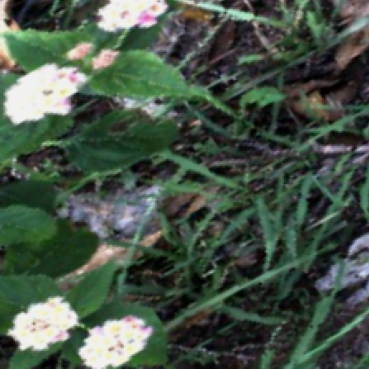
\includegraphics[width=\textwidth]{figuras/implementacion/dataset/imagenes_datagen_5.png}
        \caption{}
    \end{subfigure}
    \hfill
    \begin{subfigure}{0.3\textwidth}
        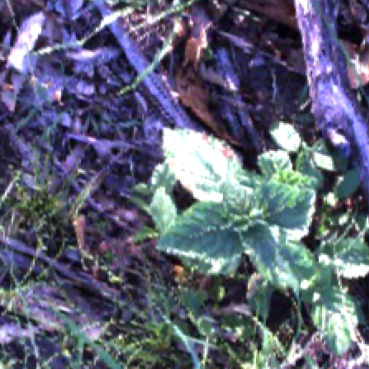
\includegraphics[width=\textwidth]{figuras/implementacion/dataset/imagenes_datagen_6.png}
        \caption{}
    \end{subfigure}
    \caption{Ejemplo de aplicación de \textit{Data Augmentation} a algunas imágenes del \textit{dataset}}
    \label{fig:datagen}
\end{figure}

\subsection{Capas Completamente Conectadas (\textit{Fully Connected Layers})}

Tras la generación de la arquitectura de la red, aún esta no está completa, ya que no tiene la capacidad de convertir la información extraída de las imágenes en las etiquetas en las que van a ser clasificadas. Por esto, se ha de añadir finalmente una estructura que sea capaz de pasar de los datos extraídos a las etiquetas de la imágenes dadas.

En este caso, se ha seleccionado la adición final de una \textbf{capa completamente conectada densa}, que tendrá el tamaño de salida del número de etiquetas de las imágenes a clasificar. Esta seguirá una función de activación \textit{softmax}, la cual normalizará la salida a una distribución de probabilidad a lo largo de las diferentes etiquetas.

\subsection{Entrenamiento por Lotes (\textit{Batch Training})}

Para la implementación realizada, se ha decidido que el entrenamiento siga un entrenamiento por lotes \cite{batch_training_edward}, el cuál está bastante estandarizado en el entrenamiento de redes neuronales. Esto es así, debido a que entrenar con conjuntos de datos completos, requiere gran cantidad de memoria, que en mucho de los casos, es imposible conseguirse. Para ello lo que se hace es entrenar con conjunto de datos más pequeños organizados en lotes en cada tiempo, lo que ocupa menor cantidad de memoria, pero también, entrena en cada tiempo con menor cantidad de datos.

El realizar este tipo de entrenamientos tiene consecuencias en función del tamaño de lote seleccionado. Un lote más pequeño, es más ruidoso, por lo que la red generaliza de peor forma. Por otro lado, un tamaño de lote más grande, tiene mayor capacidad de generalización \cite{brownlee_how_2019}.

Otra consecuencia, es el tiempo por \textit{epoch}, que para lotes más grandes, se ve reducido este tiempo de manera considerable, lo cual es adecuado para la aplicación que se está buscando, donde una pequeña diferencia temporal, finalmente pueden supone varias horas de reducción total. Es por ello, que habiendo ajustado bien el resto de parámetros, se buscará tener lotes altos \cite{chang_effect_2020}.

En este caso, se tiene bastante memoria dedicada al entrenamiento de las redes, pero no es suficiente para almacenar el \textit{dataset} completo. Es por ello que realizando diferentes pruebas del lote más alto que puede ejecutar la red, se establece que el lote con el que se entrenará es de \textbf{32} imágenes.

\subsection{Métodos de Descenso de Gradiente}

Dentro de la implementación del algoritmo del Descenso del Gradiente, existen diferentes formas de mejorar el rendimiento de este, en función del entrenamiento, persiguiendo localizar de forma eficiente y rápida los mínimos globales, evitando el estancarse en mínimos locales.

Para esto, Tensorflow facilita la implementación de diferentes técnicas que pueden ser empleadas en este caso. Las más empleadas son: \textit{Stochastic Gradient Descent} (SGD), Momentum, AdaGrad, RMSProp y Adam. A continuación, se va a realizar una rápida explicación de cada uno de estos métodos.

\begin{itemize}
    \item \textbf{SGD:} El funcionamiento básico es el ya explicado en las bases teóricas, y se basa simplemente en desplazarse en dirección contraria al gradiente de forma proporcional a este y a un \textit{learn rate} seleccionado \cite{NIPS2010_abea47ba}, al que se le añade cierta oscilación, con el que tratar de evitar el estancarse en ciertos mínimos locales, y aumentar la exploración a largo del espacio de búsqueda. Este tiene ciertos problemas cuando el los pasos del gradiente son diferentes entre las distintas dimensiones del espacio de búsqueda, ya que las oscilaciones pueden ser demasiado grandes.
    
    \item \textbf{Momentum:} Este añade la idea basada en la adición de cierta inercia al desplazamiento original del descenso de gradiente \cite{QIAN1999145}, para evitar los problemas que trae SDG. Esto hace que, debido a la velocidad acumulada en el descenso del gradiente, disminuya las oscilaciones de forma adecuada hacía la dirección del gradiente, haciendo que a la vez, se llegue de forma más rápida al mínimo.
    
    \item \textbf{AdaGrad:} A diferencia de los anteriores, este método adapta el \textit{learn rate} a cada uno de los parámetros de la red, haciendo que sea más grande el \textit{learn rate} para parámetros que se modifican en menos ocasiones y más pequeños para los que lo hacen más frecuentemente \cite{JMLR:v12:duchi11a}. Esto aumenta la robustez de la búsqueda frente a los métodos anteriormente comentados. 
    
    \item \textbf{RMSProp:} Este es una variación de AdaGrad, en el cual en vez tener acumulados todos los gradientes, se añade el concepto de la variable ``w'', la cual fija una ventana, considerando únicamente los gradientes más recientes \cite{hinton_srivastava_swersky}. Este soluciona los problemas que tiene AdaGrad, que en tiempos avanzados los pasos se hacen demasiado pequeños, lo cual hace muy lento el proceso de entrenamiento.
    
    \item \textbf{Adam:} Se trata de una combinación entre RMSProp y Momentum, donde se calcula una combinación lineal entre el gradiente y el incremento anterior, además de considerar los gradientes recientemente aparecidos para mantener diferentes tasas de aprendizaje para cada una de los parámetros de la red \cite{kingma2017adam}.
    
\end{itemize}

Una vez conocidas las cualidades \cite{DBLP:journals/corr/Ruder16} y desempeño \cite{jiang_visual_2020} de cada una de estas, y por tanto se selecciona la implementación de \textbf{Adam}, ya que este es el más extendido en la actualidad y se considera que es el adecuado para el entrenamiento de las numerosas arquitecturas que van a ir apareciendo, ya que es el que da un mejor rendimiento en términos generales a otros tipos de métodos estudiados.

\subsection{Métricas de \textit{Accuracy} y \textit{Loss}}

Para una correcta evaluación del desempeño de la red, es importante seleccionar las métricas que medirán los valores de \textit{accuracy} y \textit{loss} de la red. Existen diferentes formas de evaluarse estas, en función de que problema se esté tratando de resolver con el clasificador en cuestión \cite{dommaraju_keras_2020}.

El problema que de clasificación que se está resolviendo en este caso, es un problema multi-clase. Esto significa que se tienen más de dos clases o etiquetas a clasificar, pero que solo una de ellas se corresponderá al mismo tiempo en la imagen de entrada. Por lo tanto, no aparecerán diferentes tipos de malas hierbas en la misma imagen, sino que solo aparecerá una planta en cada imagen.

Para este tipo de problemas, se emplea el denominado \textbf{\textit{categorical accuracy}}, el cual establece cuantas imágenes se han clasificado de forma correcta del total de imágenes de esta categoría a clasificar.

Para evaluar el \textit{loss}, se va a emplear el denominado \textbf{\textit{cross-entropy loss}}, el cual es el adecuado para arquitecturas como las que se van a generar en esta implementación, donde la última capa densa, la función de activación es \textit{softmax}, ya que la red está diseñada para dar una cierta probabilidad a cada una de las etiquetas de ser el tipo de mala hierba de la imagen de entrada.

\subsection{\textit{Learn Rate} Adaptativo}

Durante el entrenamiento de una red neuronal, es posible que el \textit{learn rate}, no sea el adecuado, haciendo que no se llegue a entrenar de forma adecuada. Esto depende mucho de la arquitectura y los datos de entrenamiento, por lo que un valor fijo puede que no sea adecuado. Esto se debe a lo que ya se comentaba en la sección de las bases teóricas, y es que unos valores de \textit{learn rate} demasiado alto provoca que puede que jamás se llegué a optimizar la red a un óptimo e incluso hacer que diverja. Por otro lado un valor demasiado bajo puede hacer que el entrenamiento se haga demasiado largo, tardando mucho en alcanzar el óptimo. En las figuras \ref{fig:learn_rate}, se puede comprobar el comportamiento que se está comentando.

\begin{figure}[h]
\centering
    \begin{subfigure}{0.49\textwidth}
        \centering
        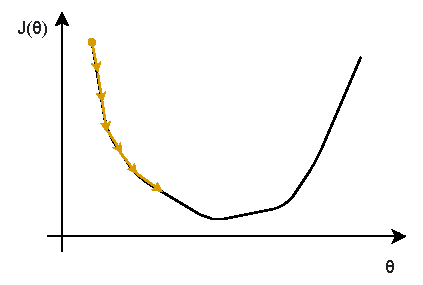
\includegraphics[width=\textwidth]{figuras/implementacion/learn rate bajo.pdf}
        \caption{\textit{Learn Rate} bajo}
        \label{fig:LR_bajo}
    \end{subfigure}
    \hfill
    \begin{subfigure}{0.49\textwidth}
        \centering
        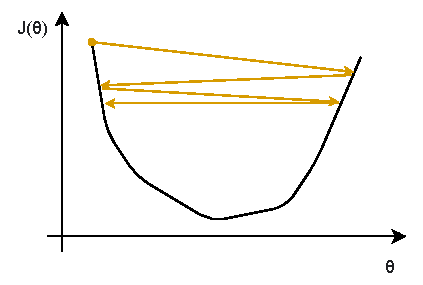
\includegraphics[width=\textwidth]{figuras/implementacion/learn rate alto.pdf}
        \caption{\textit{Learn Rate} alto}
        \label{fig:LR_alto}
    \end{subfigure}
    \hfill
    \begin{subfigure}{0.49\textwidth}
        \centering
        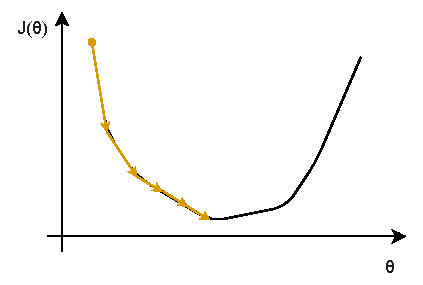
\includegraphics[width=\textwidth]{figuras/implementacion/learn rate optimo.pdf}
        \caption{\textit{Learn Rate} óptimo}
        \label{fig:LR_optimo}
    \end{subfigure}
\caption{Comportamiento en función del \textit{Learn Rate}}
\label{fig:learn_rate}
\end{figure}

Es por esto, que debido a que se tienen que entrenar numerosas arquitecturas diferentes y con diferente requerimiento, se implementa un algoritmo de \textbf{\textit{Learn Rate} adaptativo}. El funcionamiento de este se basa en el establecimiento de un \textit{Learn Rate} inicial alto. Posteriormente se debe monitorizar el error de validación. A partir de la evolución de este parámetro, se conocerá la capacidad de seguir aprendiendo de la red. Si este deja de disminuir en cierto punto, quiere decir que el \textit{Learn Rate} es demasiado alto o ha llegado a un punto óptimo. Para ello se establece un valor de \textit{paciencia}, por el cual, si el error de validación no ha disminuido en cierta cantidad de \textit{epochs}, se divide el valor de \textit{learn rate} entre dos. Así hasta que el entrenamiento haya concluido.

\subsection{Condición de parada}

Por la misma razón que se debe introducir un \textit{learn rate} adaptativo, debe establecerse una condición de parada de entrenamiento que sea variable en función de la arquitectura de la red, ya que cada una requiere mayor o menor tiempo de entrenamiento en función de sus características. Es por ello que se introduce el \textbf{\textit{Early Stopping}} \cite{Prechelt1998} dentro de la implementación realizada.

El funcionamiento de este es similar a lo que ya se veía en el \textit{Learn Rate} adaptativo. Se debe monitorizar una variable a lo largo del entrenamiento y se establece un valor de \textit{paciencia}. Esta variable ha de estar disminuyendo durante los \textit{epochs} establecidos en el valor de paciencia. Si no ha disminuido en este valor de \textit{epochs} establecido se termina el entrenamiento.

De igual manera, en este caso se va a monitorizar el error de validación durante el entrenamiento, que como ya se comentaba anteriormente, nos indica la capacidad de seguir aprendiendo que tiene la red. Además, es una forma de detectar el punto donde la red está comenzando a realizar \textit{overfitting}.

\subsection{Resolución de la Imagen de Entrada}

Debido a las limitaciones computacionales que se han resaltado durante todo el trabajo, es necesario encontrar formas de ejecutar el código de forma eficiente. Es por ello que, para agilizar el entrenamiento de las redes, se ha optado por entrenarse con imágenes de menor resolución. Esto agiliza en varios ordenes de magnitud los tiempos de entrenamiento de las redes, lo cuál permite la ejecución de este algoritmo en tiempos que hace interesante su uso en aplicaciones reales.

Esto tiene contrapartidas, y es la pérdida de información valiosa de las imágenes para su clasificación debido a la bajada de resolución de las mismas. Para ello durante la experimentación, se verificará cual es la resolución adecuada para la ejecución del Algoritmo Evolutivo, de manera que en tiempos adecuados se pueda verificar el desempeños de las diferentes arquitecturas y compararlas entre sí. 

\subsection{Entrenamiento manual posterior de los mejores individuos}

Debido a lo comentado en el apartado anterior, las redes durante la ejecución del Algoritmo Genético, se entrenan con imágenes de menor resolución. Esto nos permite descubrir arquitecturas con gran desempeño o posible potencial para clasificar las imágenes de entrada.

Esto no resulta el entrenamiento final de la red, sino que para esta se le establecen requisitos mayores, y por tanto, se debe extraer el mayor potencial de las redes. Es por ello que deben ser entrenadas posteriormente con mayor delicadeza y conciencia para que estas rindan de la mejor manera posible.

Para esto se establecen mayores tiempo de entrenamiento y condiciones de paradas más extensas. Además, la resolución de entrada de las imágenes serán de mayor tamaño, ya que las limitaciones temporales y computacionales, no son tan grandes como en las que se podrían requerir durante la ejecución del Algoritmo Genético.

Durante la experimentación se tratará de verificar que este procedimiento es adecuado, y que con entrenamientos más largos y con imágenes de entrada de mayor resolución, el desempeño de las redes crece de manera considerable, y por tanto, se extrae el potencial completo de las arquitecturas generadas.
